\documentclass[10pt,twocolumn,twoside,english,a4paper]{article}

\usepackage{placeins}
\usepackage[IL2]{fontenc} 
\usepackage[utf8]{inputenc}
\usepackage{graphicx}
\usepackage{url} 
\usepackage{hyperref} 
\usepackage{cite}
\usepackage{subcaption}
\usepackage{float}

\begin{document}
\section{Exercise 4}

\begin{figure}[h]
   \begin{minipage}[t]{1\linewidth}
     \centering
     
\includegraphics[width=1\linewidth]{STU-FIIT-ancnh.png}
     \caption{English fiit STU}\label{Fig:Data1sq}
   \end{minipage}\hfill

\end{figure}

\vspace{-1em}


\begin{figure*}[!htb]
   \begin{minipage}[t]{0.6\linewidth}
     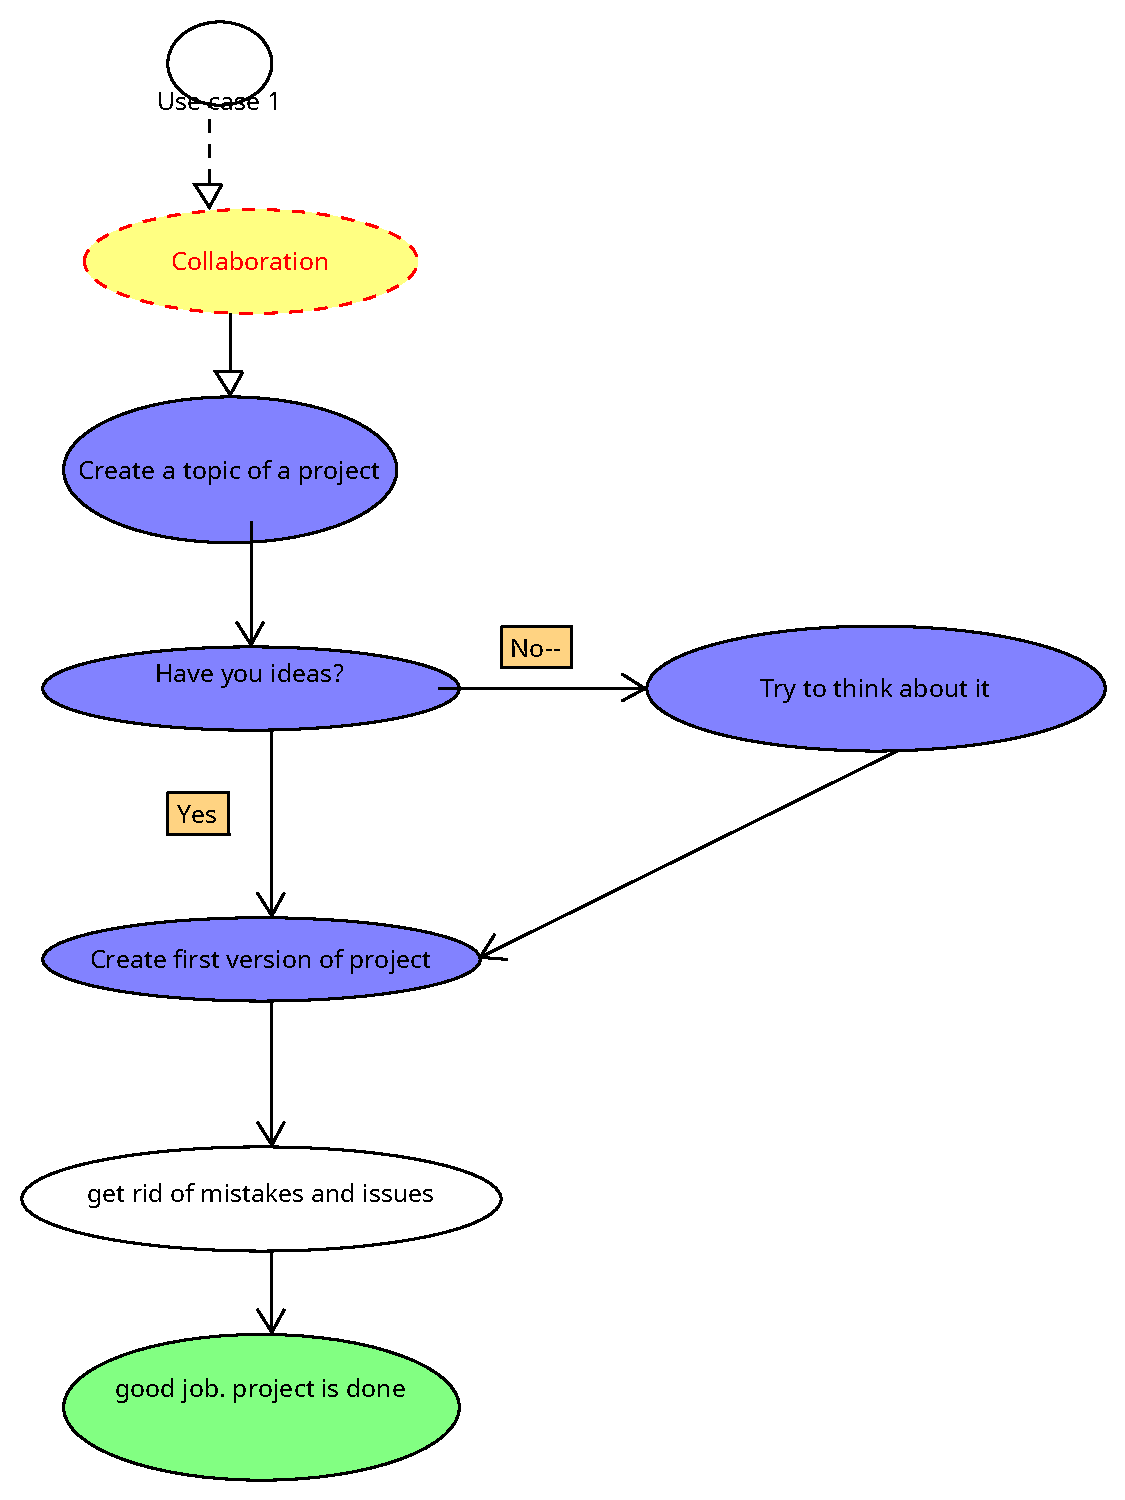
\includegraphics[width=0.8\linewidth]{graph.pdf}
     \caption{First figure in pdf}\label{Fig:Data1}
   \end{minipage}\hfill
   \begin{minipage}[t]{0.6\linewidth}
     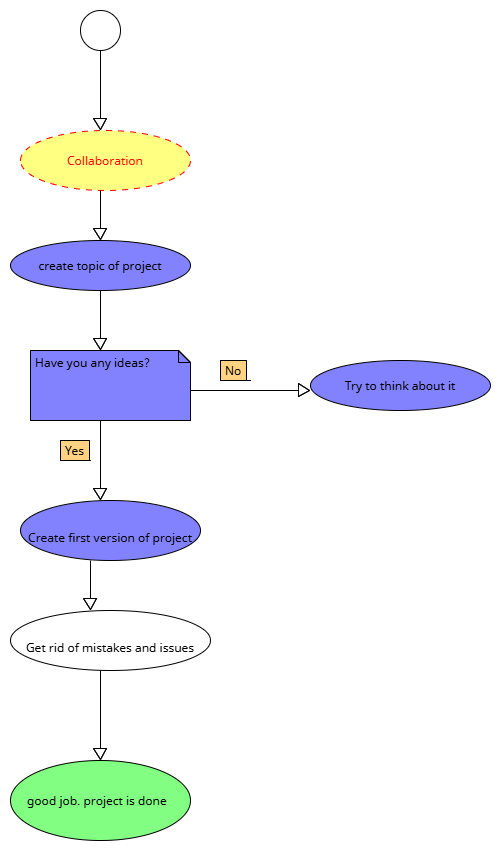
\includegraphics[width=0.7\linewidth]{graph.png}
     \caption{First figure in png}\label{Fig:Data2}
   \end{minipage}
\end{figure*}


\begin{figure*}[!htb]
   \begin{minipage}[t]{0.6\linewidth}
     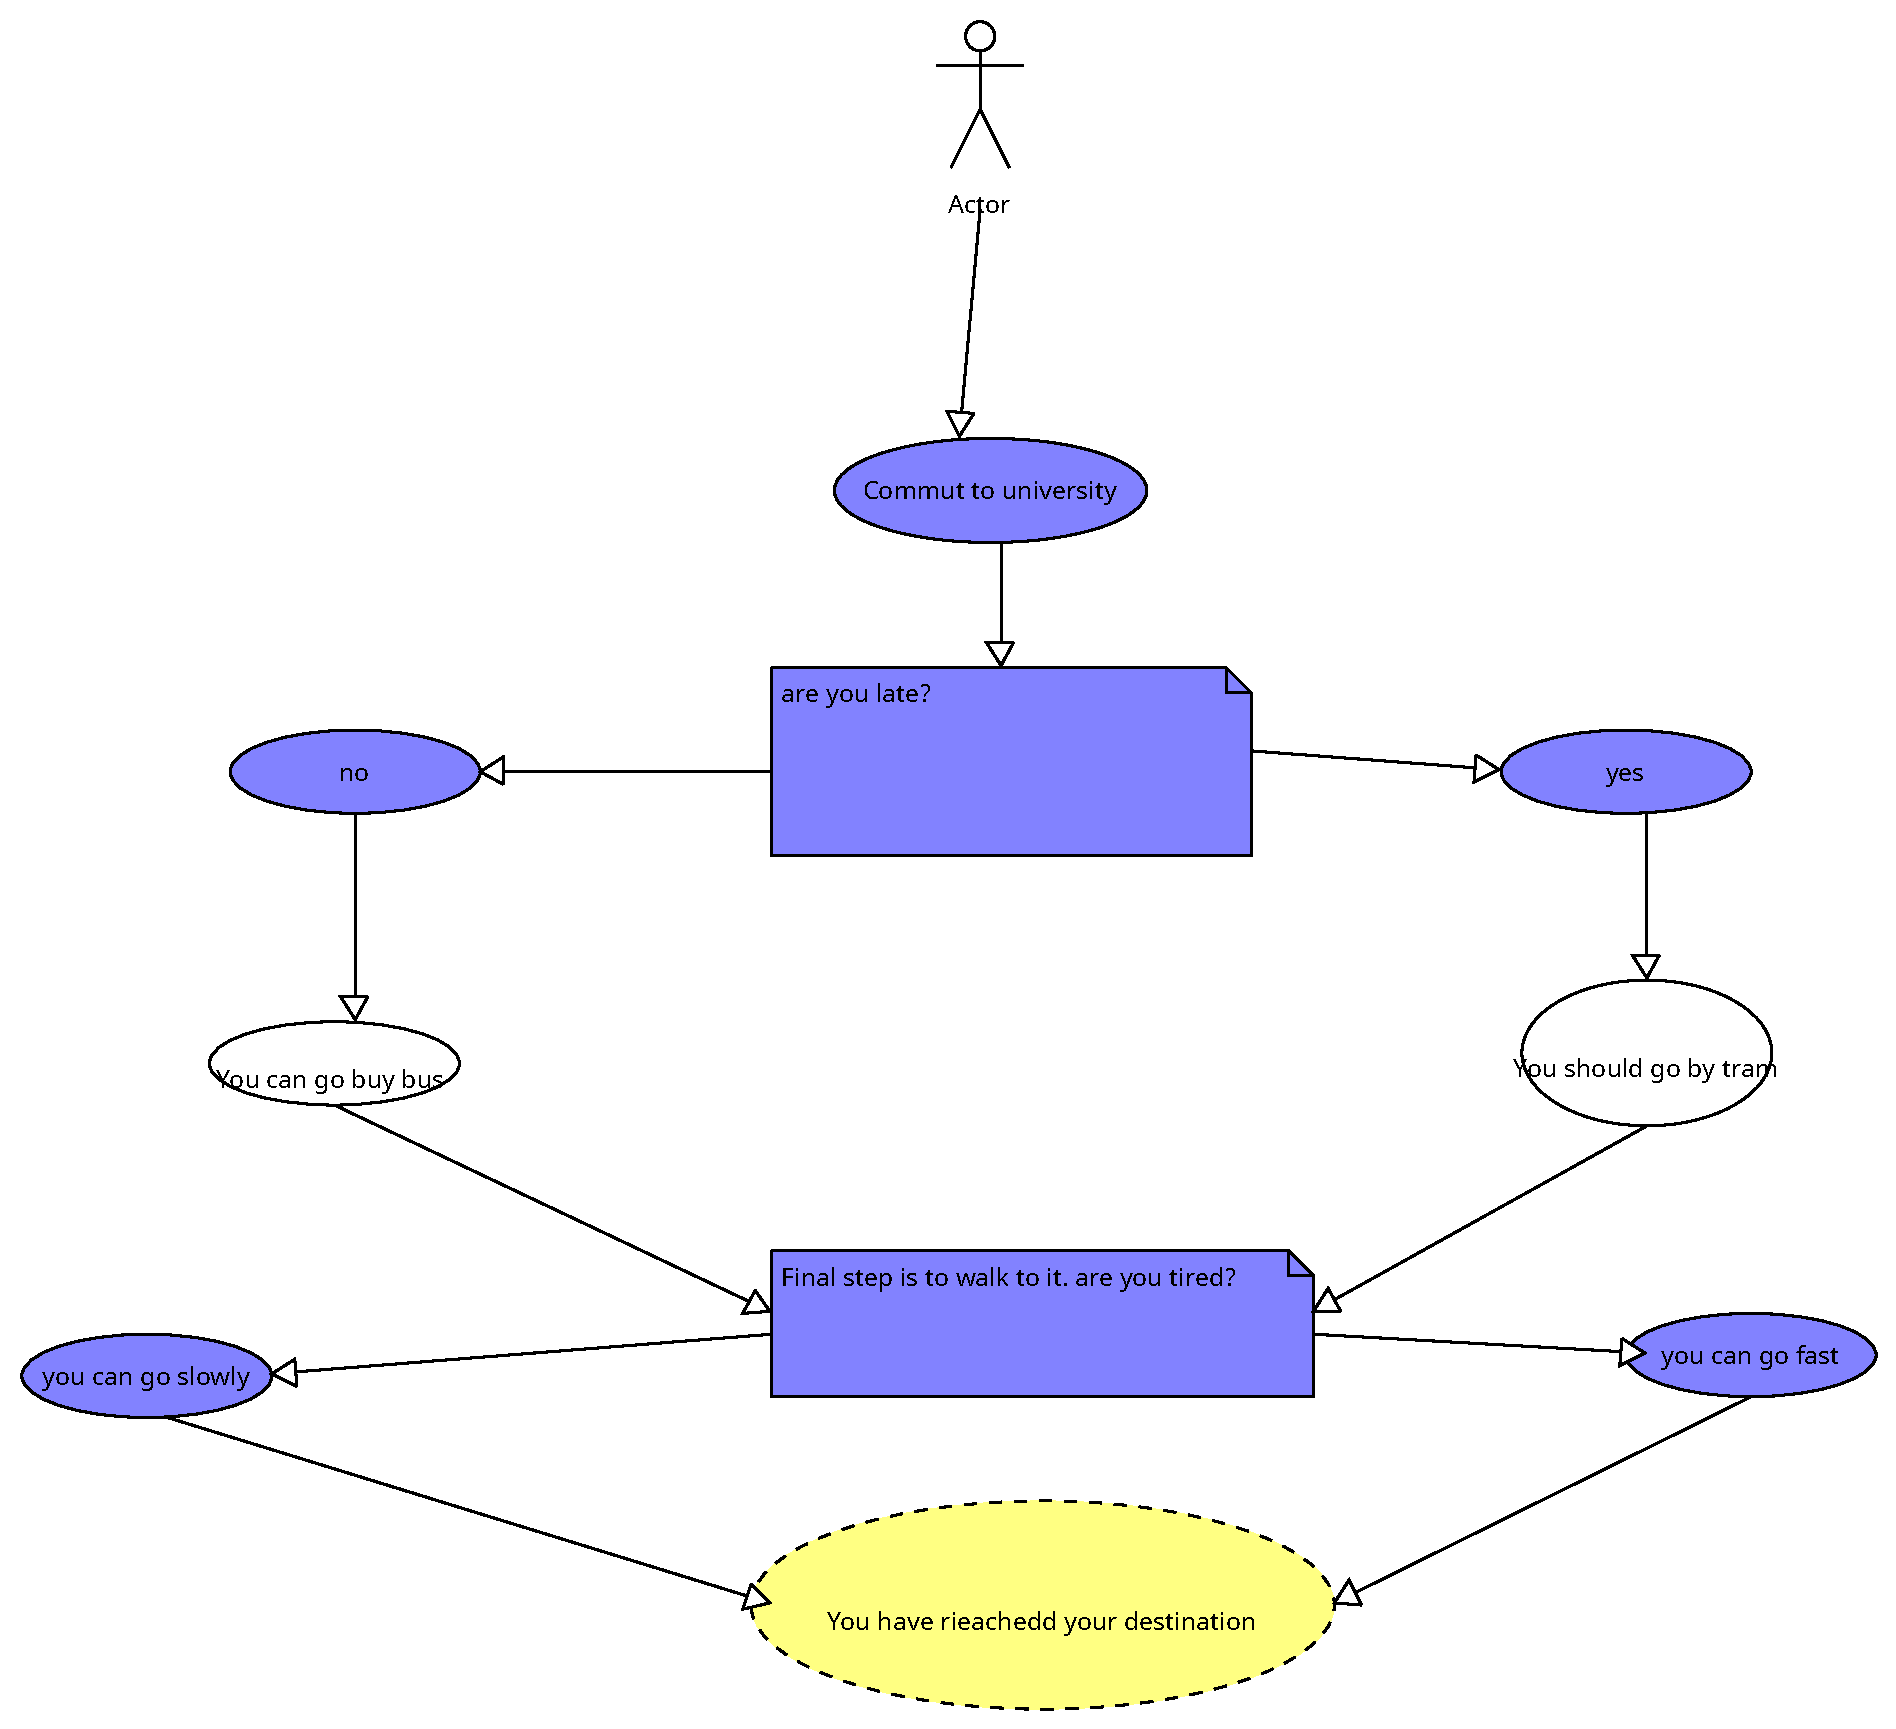
\includegraphics[width=0.8\linewidth]{diagram1.pdf}
     \caption{Second figure in pdf}\label{Fig:Data1b}
   \end{minipage}\hfill
   \begin{minipage}[t]{0.6\linewidth}
     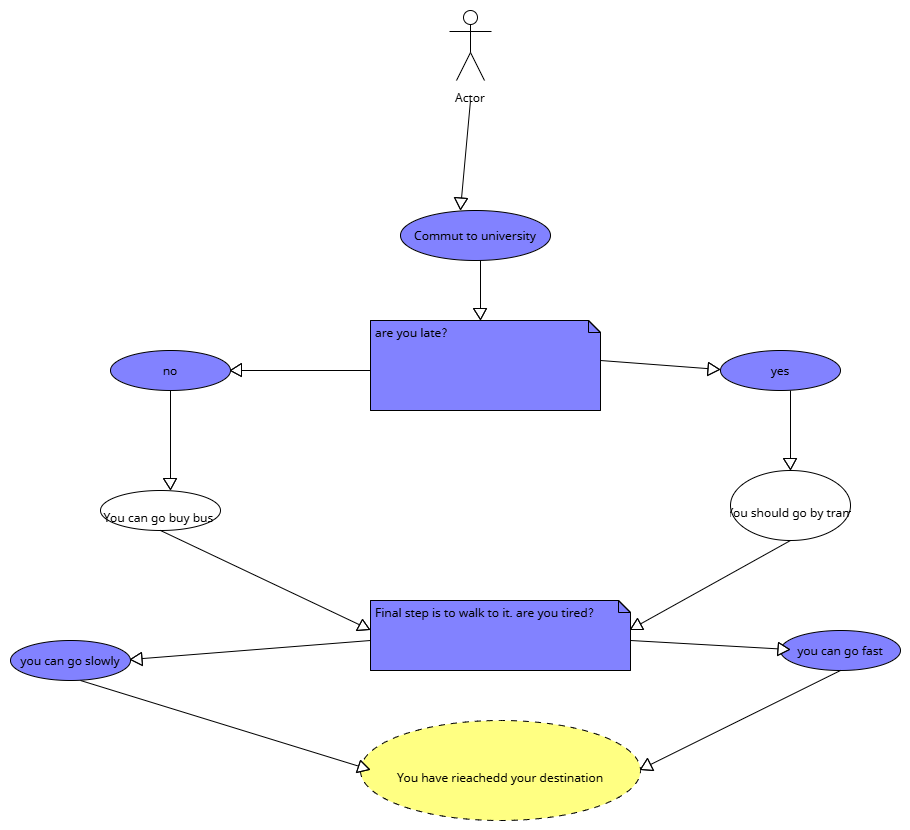
\includegraphics[width=0.8\linewidth]{diagram1.png}
     \caption{Second figure in png}\label{Fig:Data3}
   \end{minipage}
\end{figure*}

\FloatBarrier

\section{For Overleaf}


\begin{figure}[h]
   \begin{minipage}[t]{0.6\linewidth}
     \centering
     
\includegraphics[width=0.4\linewidth]{Black_square.jpg}
     \caption{figure for overleaf in pdf}\label{Fig:Data1sq}
   \end{minipage}\hfill

\end{figure}

\mbox{}

\end{document}

